\documentclass[11pt]{article}
\usepackage[utf8]{inputenc}

%Don't change any thing before \begin{document}
%They are not useful for now, but later when you try to add figures
%these might be useful. In fact if you use sth fancy, you might need
%to add more packages, or macros.
\usepackage{amssymb,amsmath}
\usepackage{times,psfrag,epsf,epsfig,graphics,graphicx}
\usepackage{algorithm}
\usepackage{algorithmic}
\usepackage{xcolor}


\title{CSCI 338: Assignment~2~(7 points)}
\author{William Jardee}
\date{}

\begin{document}

\maketitle
 
\section*{Problem 1.}

\noindent
\textbf{1.1} Problem 1.6d, 1.6e:\\
Give a state diagram of a DFA that recognizes:\\

\textbf{(1.6d)}
    \begin{center}
        $\{\omega | \omega$ has length at least 3 and its third symbol is a 0 $\}$.\\
        \bigbreak
        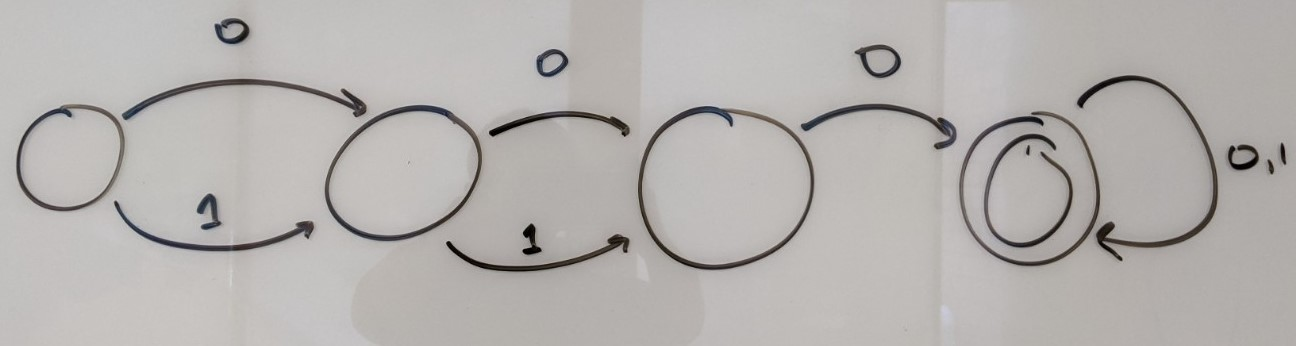
\includegraphics[width = .9\textwidth]{images/homework02/answer1.6d.jpg}\\
    \end{center}
\bigbreak
\textbf{(1.6e)}
    \begin{center}
        $\{\omega | \omega$ starts with 0 and has odd length, or starts with 1 and has even length$\}$\\
        \bigbreak
        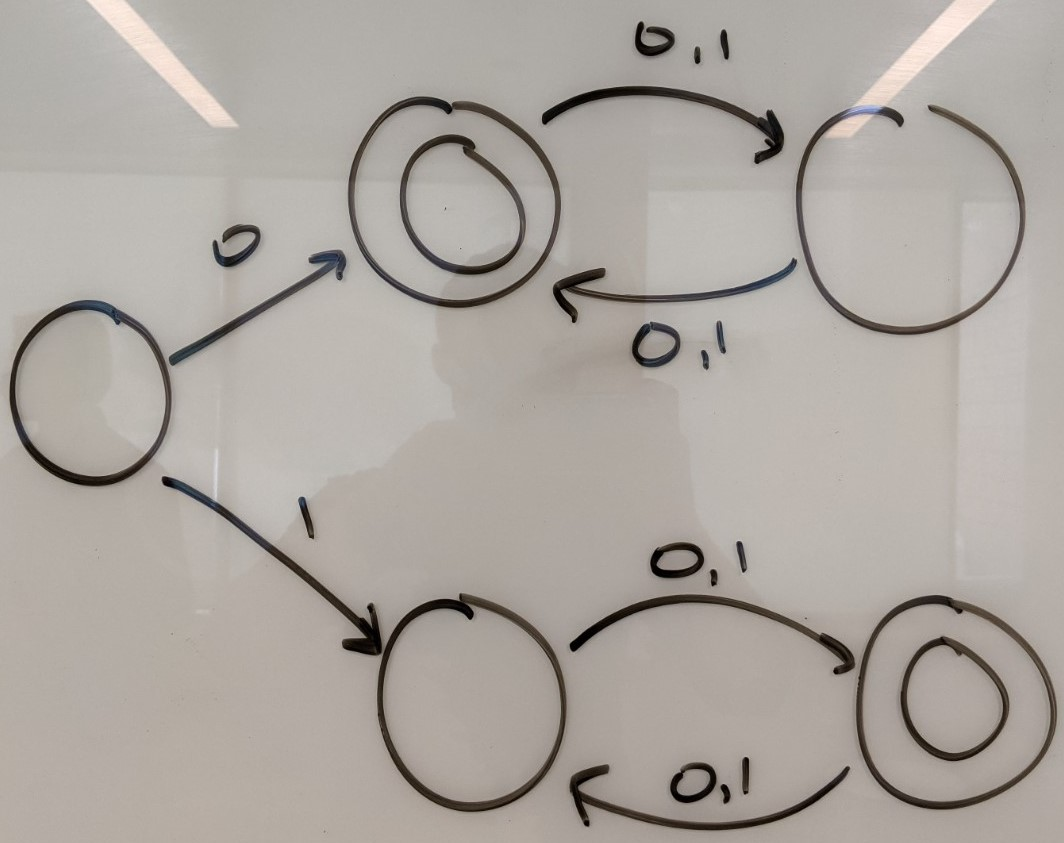
\includegraphics[width = .55\linewidth]{images/homework02/answer1.6e.jpg}\\
    \end{center}

\newpage




\noindent
\textbf{1.2} problem 1.7b, 1.7c:\\
Give a state diagram of a NFA that recognizes:\\

\textbf{(1.7b)}
    \begin{center}
        $\{ \omega | \omega$ contains the substring 0101 (i.e., $\omega = x0101y$ for some $x$ and $y\}$ with only five states.\\
        \bigbreak
        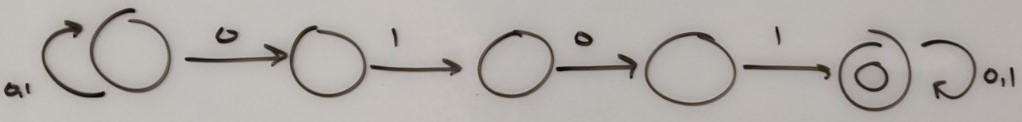
\includegraphics[width = .9\linewidth]{images/homework02/answer1.7b.jpg}\\
    \end{center}
\bigbreak
\textbf{(1.7c)}
    \begin{center}
        $\{\omega | \omega$ contains an even numbers of 0's, or contains exactly two 1's$\}$ with only six states.\\
        \bigbreak
        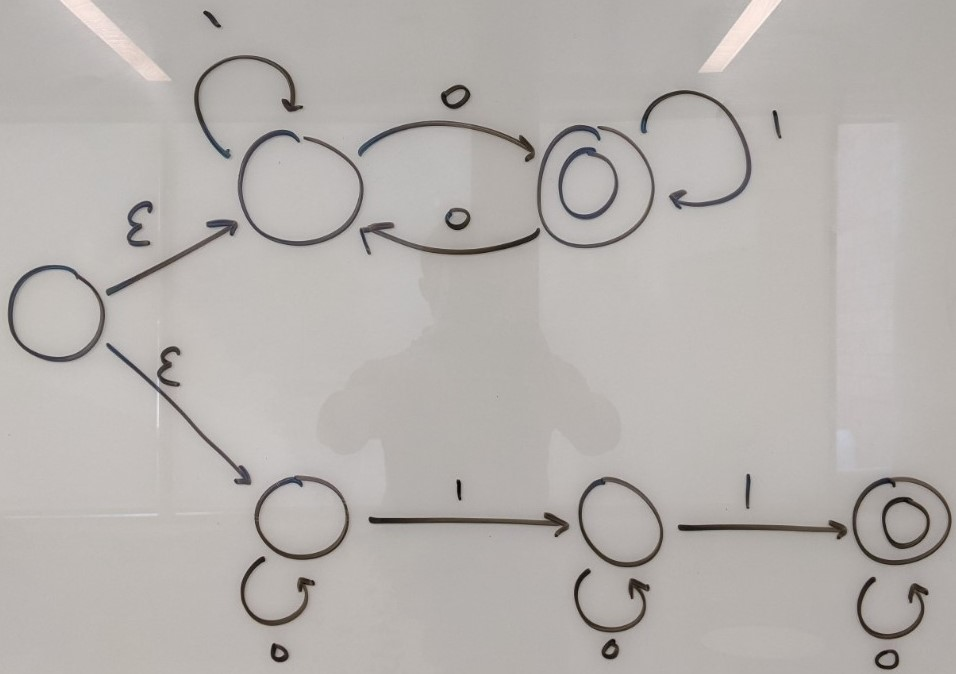
\includegraphics[width = 0.8\linewidth]{images/homework02/answer1.7c.jpg}\\
    \end{center}

\newpage





\section*{Problem 2.}
Do problems 1.16a and 1.16b.\\
Convert the following NFA to equivalent DFA.\\

\textbf{(1.16a)}
\begin{center}
    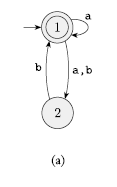
\includegraphics[width = .2\linewidth]{images/1.16a.PNG}
    \hspace{.1\linewidth}
    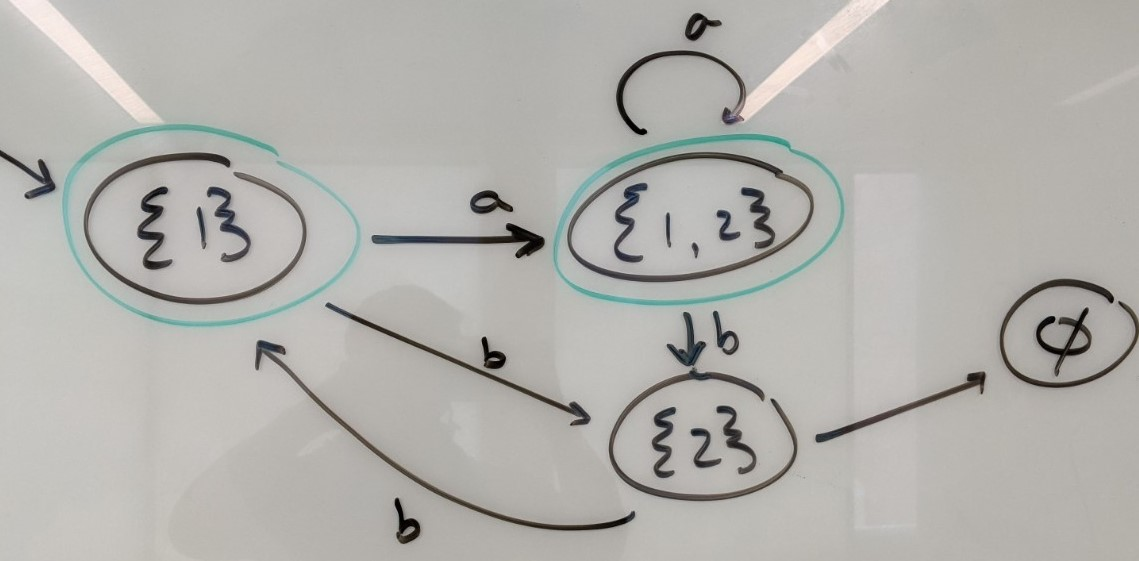
\includegraphics[width = .6\linewidth]{images/homework02/answer1.16a.jpg}
\end{center}


\textbf{(1.16b)}
\begin{center}
    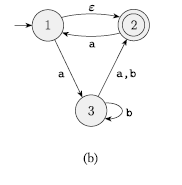
\includegraphics[width = .3\linewidth]{images/1.16b.PNG}
    \hspace{.1\linewidth}
    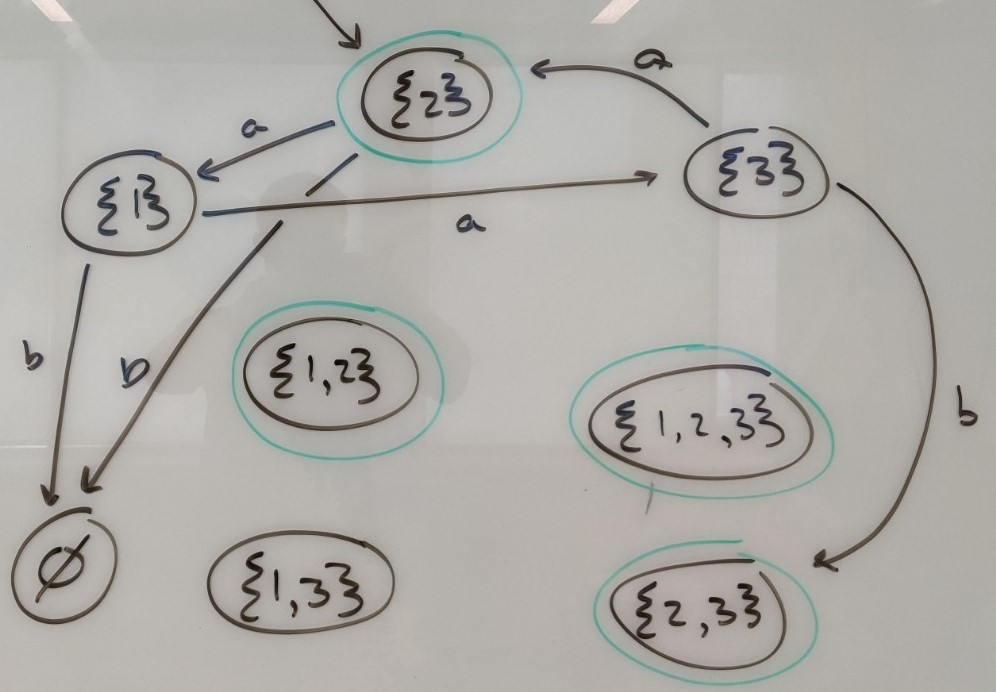
\includegraphics[width = .5\linewidth]{images/homework02/answer1.16b1.jpg}\\
    \bigbreak
    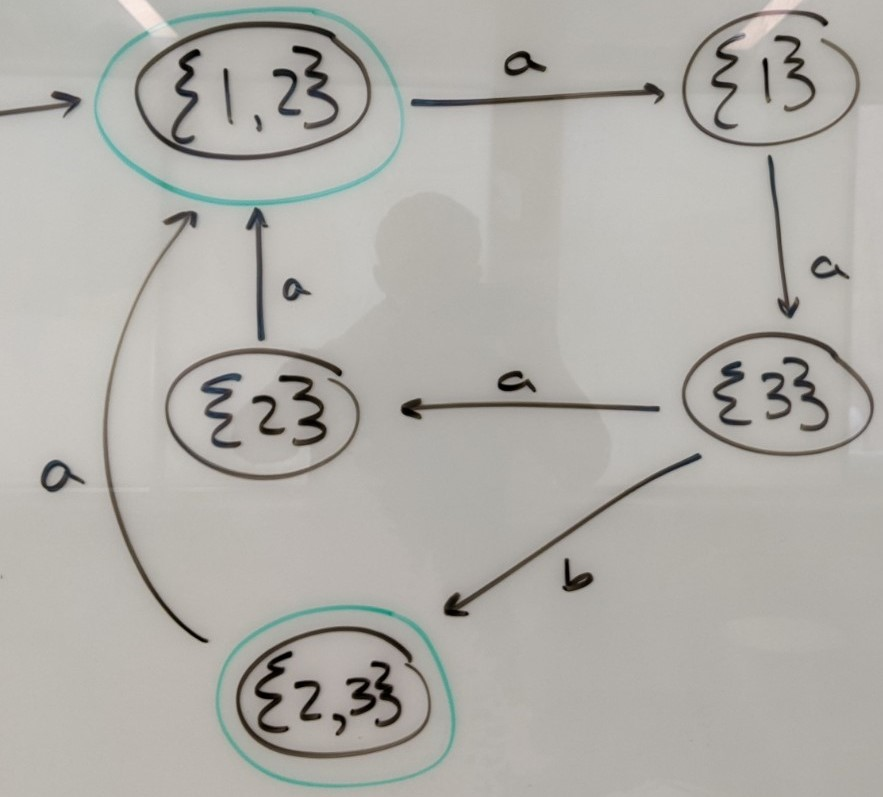
\includegraphics[height = 150pt]{images/homework02/answer1.16b2.jpg}\\
\end{center}

\newpage




\section*{Problem 3.}
Do Problems 1.19a and 1.19b.\\
Convert the following regular expressions to NFA.\\

\textbf{(1.19a)} $(0\cup 1)^* 000 (0\cup 1)^*$
\begin{center}
    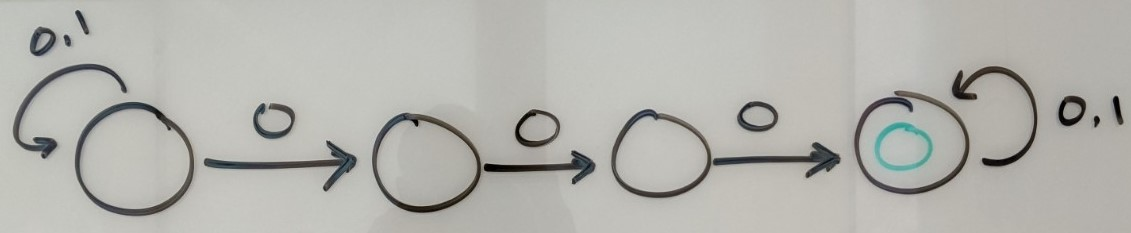
\includegraphics[width = 0.9\linewidth]{images/homework02/answer1.19a.jpg}
\end{center}

\textbf{(1.19b)} $(((00)^*(11))\cup 01)^*$
\begin{center}
    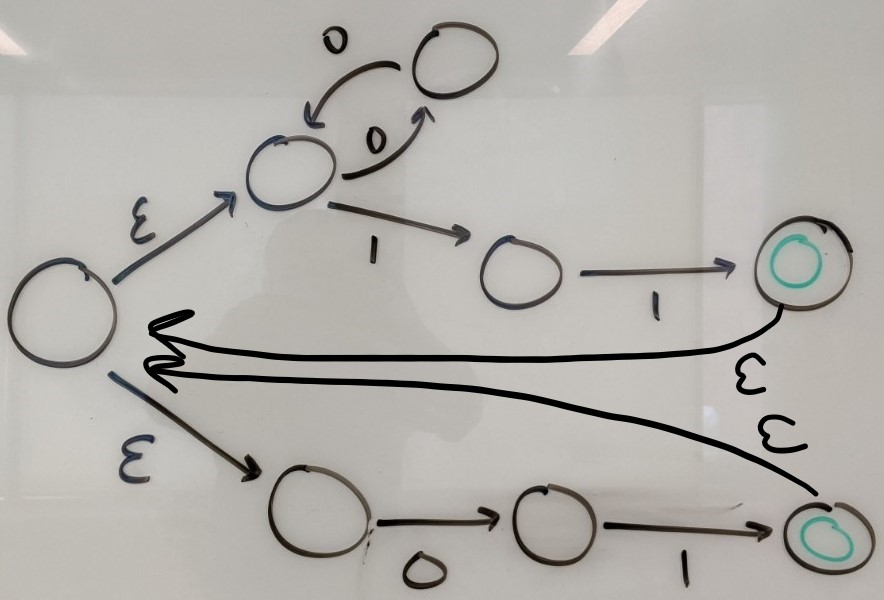
\includegraphics[width = 0.7\linewidth]{images/homework02/answer1.19b.jpg}
\end{center}

\newpage





\section*{Problem 4.}
Problem 1.21a:\\
    Convert the following DFA to a regular expression.\\
    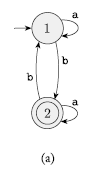
\includegraphics[height = 150pt]{images/1.21a.PNG}\\
    I applied the process where we ``rip" out a node, in this case we remove node 1, and replace the transition with the equivalent $R_{11}^* R_{12} (R_{22} \cup R_{21}R_{11}^*R_{21})^*$. Here $R_{11} = R_{22} = a$, $R_{12} = R_{21} = b$.
    \begin{center}
        \boxed{a^* b(a\cup ba^* b)^*}
    \end{center}
\newpage





\section*{Problem 5.}
Prove the following languages are not regular.\\

\textbf{(5.1)} $A=\{a^{n^3}|n\geq 0\}$ Here $a^x$ means a string of $x a$'s.\\

\textbf{Proof by Contradiction:}

Let us start by assuming that A is a regular language so we can apply the pumping lemma to A. I will assume that we know what this lemma does and simply use it. First, let's rewrite $A = \{a^n a^n a^n | n \geq 0\} = \{a^{3n} | n\geq 0 \cap n \in \mathbb{Z}\}$ (to be more complete, we must say that $n\in \mathbb{Z}$). If we have some pumping length $P$, then there must be some structure $xy^i z$ that is always valid in A. What this means is that $A = a^P a^{3n-P}$ and that every $A = a^{\alpha P} a^{3n-P} = a^{3n + (\alpha-1)P} = a^{(n+\frac{(\alpha -1)P}{3})^3} = a^{\beta^3}$, such that $\beta = \frac{(\alpha-1)P}{3}$, are valid. However, the integers are not closed under division, so there is no guarantee that $\beta$ is an integer, meaning that we could have a string with a non-integer length. This, obviously, cannot exist, so we have run into a contradiction. So, $A=\{a^{n^3} | n\geq 0\}$ is not a regular language.
\begin{flushright}$\blacksquare$\end{flushright}

\textbf{(5.2)} $B=\{0^n 1^m 0^n | m,n \geq 0\}$\\

\textbf{Proof by Contradiction:}

Let us start by assuming, for the point of contradiction, that $B$ is a regular language. Then we can apply the pumping lemma to $B$, stating that there must be some $xy^i z$, s.t. $i\in \mathbb{Z}$, that is always valid in $B$. I will cover three base examples of applying the pumping lemma, and all other choices of $x$, $y$, and $z$ fall under the same contradictions. \\

\textbf{1.} Let $P=n$, such that $xy^i = 0^P = 0^n$. Then we get that $B=\{0^P 1^m 0^n | m,n \geq 0\}$ and that $B$ must contain $0^P 0^P 1^m 0^n = 0^P 0^P 1^m 0^P$. This obviously can't be true, so we must look for another $P$ then. \textit{Notice that if I chose $P=n/2$, and forced $n$ to be even, that we run into the same issue. }\\

\textbf{2.} Let $P=n+m$, such that $xy^i = 0^n 1^m \leq P$. Then we get that $0^n 1^m 0^n 1^m 0^n$ must exist in $B$, which is not a valid statement.\\

\textbf{3.} Finally, let $P=n+m+n$, such that $xy^i = 0^n 1^m 0^n \leq P$. Then $0^n 1^m 0^n 0^n 1^m 0^n$ must exist in $B$, which is not true.\\

Any other choice of $x$, $y$, and $z$ will fall into some combination of the previous contradictions, as any choice will be a subset of those already covered. For this reason, we can say that there are no choice that holds with the pumping lemma and, through contradiction, $B=\{0^n 1^m 0^n | m,n \geq 0\}$ is not a regular language. 
\begin{flushright}$\blacksquare$\end{flushright}



\end{document}
